Appendices
\newline
http://www.prasannatech.net/2008/07/socket-programming-tutorial.html
Domain Specific Languages
\newline
style of programing ( language oriented programming ) Sergey Dmitrov
\newline
general purpose programming languages
\newline
small and limited languages ( dsls )
\newline
unix languages, lisp, macros
\newline
xml
\newline
data in text file, each line is an event, event data
\newline
parse event data an turn into usefull events
\newline
fuzzy distinction ( within the language )
\newline
attitue to design
\newline
external
\newline

-separate to the host language
\newline

-needs a compiler / interpreter to execute
\newline

-tied to base language
\newline

-awkward with mainstream { languages }
\newline
internal
\newline

-written in the host language
\newline

-conventional use of host language syntax
\newline

-Lack of Symbolic Integration
\newline

-complex parser / generator technologies
\newline

-Ignorant IDEs
\newline

-language cacophany
\newline
custom language to understand complex instructions
\newline
you have to problem anyway
\newline
DSL will provide simpler solution Patterns
\newline
\url{http://en.wikipedia.org/wiki/You_ain't_gonna_need_it}
\newline
\url{http://www.dofactory.com/Patterns/PatternStrategy.aspx}
\newline
\url{http://www.perl.com/pub/2003/08/07/design2.html}
Perl Filters 
\newline
\url{http://linux.about.com/library/cmd/blcmdl1_perlfilter.htm}    
\newline
\url{http://www.coderaptors.com/?Perl_Source_Filters}
\newline
\url{http://www.kichwa.com/quik_ref/spec_variables.html}
\newline
Domain specific languages are not a new concept.  They have been around since unix and lisp.
\newline
generic and specific approaches
\newline
generic approach is sub optimal
\newline
dichotomy - A division or contrast between two things that are or are represented as being opposed or entirely different.
\newline
dedicated language for solving problem in specific 
\newline
business processing, numeric computation and symbolic processing
\newline
evolving into general purpose languages
\newline
resurfaced of DSL's to solve domain specific problems resurfacing
\newline
subroutines to handle domain problems
\newline
OO frameworks with application specific code
\newline
Arie van Deursen Paul Klint Joost Visser 
"A domain-specific language (DSL) is a small, usually
declarative, language that offers expressive power focused
on a particular problem domain. In many cases,
DSL programs are translated to calls to a common subroutine
library and the DSL can be viewed as a means to
hide the details of that library."
\newline
semantic study of DSLS
\newline
terminology
\newline
risks and opportunities
\newline
example DSLs
\newline
DSL design methodology and DSL implementation strategies
\newline
importance of DSLS
\newline
Arie van Deursen Paul Klint Joost Visser 
"A domain-specific language (DSL) is a programming
language or executable specification language
that offers, through appropriate notations and abstractions,
expressive power focused on, and usually
restricted to, a particular problem domain."
\newline
expressive power
\newline
vagueness of the problem domain
\newline
domain modelling
\url{http://www.program-transformation.org/Transform/OrganizationDomainModeling}
\newline
DSLs are usually small, offering only a restricted suite of
notations and abstractions
\newline
Domain specific expressive power with Power of embedded General purpose language , known as embedded languages ( fowler alternative )
\newline
power restricted to problem domain
\newline
declarative seen as specific languages
\newline
DSL compiler known as application generator ( make reference to perl filter and how admin is not required to learn a further technology by use of a transformation into the intended language in which is was design ed and or implemented from )
\newline
application specific language
\newline
4th generation language ( 4gl) business data processing systems
\newline
balance between risk and opportunities. 
argue here that providing a filter as opposed to a compiler it allows the admin to take off from where the specification left off
\newline
extensibility, allow for the developed of the DSL, as the domain is user expressed
\newline
enhance productivity, reliability, maintainability, portability
\newline
"Domain-specific languages (DSLs) have the potential
to make software maintenance simpler: domain-experts
can directly use the DSL to make required routine modifications.
At the negative side, however, more substantial
changes may become more difficult: such changes
may involve altering the domain-specific language. This
will require compiler technology knowledge, which not
every commercial enterprise has easily available. The
paper describes and uses the experience of the RISLA
language for interest rate products to discuss the role of
DSLs in software maintenance, the opportunities introduced
by using them, and techniques for controlling the
risks involved."
\newline
argue here that providing a GPL abstract with  transformation engine, expressing that fowler said 'what the bloddy hell that lecturer was on about back in college about compilers, parse tress and grammer'
\newline
R. B. Kieburtz, L. McKinney, J. M. Bell, J. Hook,
A. Kotov, J. Lewis, D. P. Oliva, T. Sheard, I. Smith,
and L. Walton. A software engineering experiment in
software component generation. In Proceedings of the
18th International Conference on Software Engineering
ICSE-18, pages 542–553. IEEE, 1996.
Reports the results of an experiment in which a templatebased
approach and a DSL approach to software generation
were compared. Several subjects were monitored
while performing a number of development and maintenance
tasks using alternatively template technology and
DSL technology. Flexibility, productivity, reliability, and
usability were measured. The DSL approach scored better
on all counts.
\newline
much like group policy providing registry updates, dsl will provide optimzation at the domain levels
\newline
cost of maintaining the DSL. constructsa of the language should be module specific but follow general over flow and try to integrate resuability and common words.
\newline
reason for this that as the domain changes as it invariably does in the linux env, so will have the DSL and will incur over head of modifying the DSL as a whole.  Common terms should implment the same behaviour however specific terminonaly to a specific problem should be component based
\newline
cost of educating 
\newline
limited availability
\newline
scoping the DSL
\newline
balance between GPL and DSL  constructs
\newline
C. W. Krueger. Software reuse. ACM Computing Surveys,
24(2):131–183, June 1992.
\newline
Categorizes, describes and compares existing approaches
to software reuse, among which DSLs (or
application generators). Compared to the other approaches
DSLs reduce the intellectual effort required to
obtain an executable system from its specification. Limited
availability and difficulty of building DSLs of optimal
specificity/generality are listed as disadvantages of
DSLs.
\newlineT
he potential loss of efficiency when compared with
hand-coded software.
\newline
possibly talk about the proficiency of PERL as a text processor
\newline
examples of DSLS
\newline
pic, scatterm chem, lex, yacc and make 
SQL, BNF and html, xml
\newline
behavior and control
control and coordination [9, 10]
F. Bertrand and M. Augeraud. BDL: A specialized language
for per-object reactive control.
\newline
Design Methodology

Analysis (1) 
Identify the problem domain. (2) Gather all relevant
knowledge in this domain. (3) Cluster this knowledge
in a handful of semantic notions and operations on
them. (4) Design a DSL that concisely describes applications
in the domain.

Implementation (5) Construct a library that implements the
semantic notions. (6) Design and implement a compiler
that translates DSL programs to a sequence of library
calls.

Use (7) Write DSL programs for all desired applications and
compile them


DSL Implementation

Interpretation or compilation
Embedded languages / domain-specific libraries
Preprocessing or macro processing
Extensible compiler or interpreter

Apart from building a dedicated DSL compiler or interpreter,
or reusing the implementation of an underlying base
language, other implementation techniques may be used. For
instance, in aspect-oriented programming [46] a DSL is used
to describe an aspect of a system’s behavior that is orthogonal
to its main functionality. An aspect weaver is then used
to generate domain-specific code and merge it with the main
code.


Programming language technology
\newline
\url{http://en.wikipedia.org/wiki/Eric_Schmidt}
\newline
\url{http://en.wikipedia.org/wiki/Context-free_grammar}
\newline
\url{http://en.wikipedia.org/wiki/Metasyntax}
\newline
\url{http://en.wikipedia.org/wiki/Bash_(Unix_shell)}
\newline
\url{http://en.wikipedia.org/wiki/Yacc}
\newline
\url{http://en.wikipedia.org/wiki/GNU_bison}
\newline
\url{http://en.wikipedia.org/wiki/Lex_programming_tool}
\newline
\url{http://en.wikipedia.org/wiki/Flex_lexical_analyser}
\newline
\url{http://en.wikipedia.org/wiki/Lexical_analysis}
\newline
\url{http://en.wikipedia.org/wiki/Backus-Naur_form}
\newline
\url{http://en.wikipedia.org/wiki/Reentrant_(subroutine)}
\newline
\url{http://en.wikipedia.org/wiki/SLR_grammar}
\newline
\url{http://en.wikipedia.org/wiki/LL_parser}
\newline
\url{http://en.wikipedia.org/wiki/GLR_parser}
\newline
\url{http://en.wikipedia.org/wiki/Finite-state_machine}
\newline
\url{http://en.wikipedia.org/wiki/LR_parser}
\newline
\url{http://en.wikipedia.org/wiki/LALR}
\newline
How to Write a Simple Parser by Ashim Gupta
\newline
\url{http://ashimg.tripod.com/Parser.html}
\newline
\url{http://hivearchive.com/2007/06/10/regular-expressions-lisp-sql-parsing-domain-specific-languages/}
\newline
\url{http://unicode.org/glossary/}


Directory Services
\newline
\url{http://en.wikipedia.org/wiki/Directory_service}
\newline
\url{http://en.wikipedia.org/wiki/X.500}
Comparison of Directory Services Solutions
\newline
Microsoft Active Directory
\newline
Windows NT Directory Services
\newline
Novell eDirectory
\newline
Red Hat Directory Server
\newline
Apple Open Directory
\newline
Apache Directory Server
\newline
Oracle Internet Directory
\newline
CA Directory
\newline
Alcatel-Lucent Directory Server
\newline
Sun Java System Directory Server
\newline
OpenDS
\newline
IBM Tivoli Directory Server
\newline
Siemens DirX Directory Server
\newline
Critical Path Directory Server
\newline
OpenLDAP
\newline
Isode Limited
\newline
UnboundID Directory Server
\newline
Lotus Domino

LDAP Data Interchange Format
\newline
\url{http://en.wikipedia.org/wiki/LDAP_Data_Interchange_Format}
\newline
RFC 2849 -  The LDAP Data Interchange Format (LDIF) - Technical Specification
\newline
RFC 4510 - Lightweight Directory Access Protocol (LDAP): Technical Specification Road Map -           
RFC 4525 — LDAP Modify-Increment Extension
Directory Services Markup Language
\newline
\url{http://en.wikipedia.org/wiki/Directory_Service_Markup_Language}

Metadirectory
\newline\url{http://en.wikipedia.org/wiki/MetaDirectory}

Virtual directory
\url{http://en.wikipedia.org/wiki/Virtual_directory}

Group policy
\newline\url{http://en.wikipedia.org/wiki/Group_Policy}

		\newline
		\newline
		Since the conception of X.500 Directory Services specification eventually leading to Microsoft’s dominance in the
	    enterprise management, there has been a continual drive to integrate mixed environments into Active Directory.  
		However due to the mixed philosophies and therein the different distributions of Open Source Software (OSS) 
		operating systems, creating policies within active directory that can manage this diversity is seen as next to 
		impossible or at least limited.  
		\newline
		\newline
		Unlike Microsoft clients that implement a common integrating architecture this cannot be said for 
		Open Source Software (OSS) systems.  
		\columnbreak
		Enterprise solutions targeting systems such as Redhat Enterprise Linux and Suse Enterprise Linux aid 
		production administrators in provisioning and maintainability but not subscribe to non - production environments 
		where a greater degree of flexibility is expected within the environment or do they employ user friendly common 
		language as seen in the windows domain.  
		\newline
		\newline
		Observations within the field have led to the rapid development of Samba 4 offering directory services allowing 
		for Windows Policies to be integrated into the internal directory structure but as of yet still no viable solution 
		for Linux polices on the horizon.
		\newline
		\newline
		 
		
		\newline
		\newline
		{\bf 2)} How these varying systems and their configurations can be represented by means of a directory services schema. 
		Like that of its Windows Group Policy Object (GPO) counterpart, the configuration, changeability and extensibility 
		of these policies through the use of the schema, should be applicable to all these systems. 
		
		
		
		
					%\vspace{5mm}
			%\normalsize
			%{
			%	The kiviat diagram Fig.\ref{fig:kiviat} shows the spread of these metrics.  The digram indicate
			%	that some section of the code have high branching and resulting complexity.  Also further commenting 
			%	is needed as with a possible reduction in documentation ( eg. JavaDoc ).
			%	\newline
			%	\newline
			%}
		
		\end{multicols}	
			
		%\vspace{-5mm}
		%\begin{figure}[h!]
		%	\centering
		%	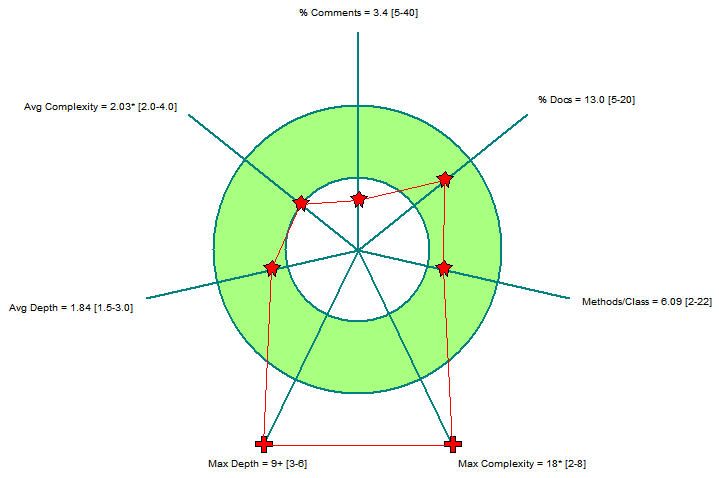
\includegraphics[scale=0.8]{figures/kaviatmetrics.png}
		%	\vspace{-2mm}
		%	\caption{Kaviat diagram}
		%	\label{fig:kiviat}
		%\end{figure}	
		
		
		
		
		
		
		
		
		
		
		
		
		
		
		
		
		

